% !TeX program = pdflatex
% =============================================================================
% Arbeitsblatt: Durchschnitts- vs. Momentangeschwindigkeit (Zusatzblatt)
% Kantonsschule KFR -- Physik, 4. Klasse, 1. HS, Mechanik / s-t-Diagramm
%
% Vertiefendes Zusatzblatt zum Hauptblatt s-t-diagramm-arbeitsblatt.tex
% (dort bereits LZ4 Durchschnittsgeschwindigkeit als Sekante, LZ8/LZ9
% Momentangeschwindigkeit/Tangente/Grenzwert eingefuehrt). Dieses Blatt
% vertieft denselben Begriffsunterschied an zwei neuen Kontexten
% (Blitzer/Abschnittskontrolle, Marathon) statt ihn neu herzuleiten.
% =============================================================================
\documentclass[addpoints,11pt,a4paper]{exam}

\usepackage[T1]{fontenc}
\usepackage[utf8]{inputenc}
\usepackage[ngerman]{babel}
\usepackage{lmodern}
\usepackage[a4paper,margin=2.2cm,headheight=14pt]{geometry}
\usepackage{amsmath}
\usepackage{siunitx}
\sisetup{per-mode=fraction,fraction-command=\frac}
\usepackage{array,booktabs,tabularx,multirow}
\usepackage{enumitem}
\usepackage{graphicx}
\usepackage{xcolor}
\usepackage{colortbl}
\usepackage{tikz}
\usepackage{physics}
\usepackage{circuitikz}
\usepackage[most]{tcolorbox}
\usepackage{lastpage}
\usepackage{needspace}

\usetikzlibrary{arrows.meta,calc,angles,quotes}

\usepackage{setspace}
\setlength{\parindent}{0pt}
\setlength{\parskip}{0.6em}
\setstretch{1.08}
\setlist[itemize]{itemsep=0.4em}

% -----------------------------
% Farben (Corporate-Farbschema Physik KFR)
% -----------------------------
\definecolor{titleblue}{HTML}{183A6B}
\definecolor{accentblue}{HTML}{2E6F9E}
\definecolor{lightblue}{HTML}{EAF4FB}
\definecolor{verylightblue}{HTML}{F7FBFE}
\definecolor{lightgray}{HTML}{F4F6F8}
\definecolor{darkgray}{HTML}{4A4A4A}
\definecolor{accentorange}{HTML}{D9720C}
\definecolor{accentpurple}{HTML}{7B2D8E}
\definecolor{theorygreen}{HTML}{2E7D4F}
\definecolor{lighttheorygreen}{HTML}{EAF7EF}
\definecolor{groupteal}{HTML}{1B7F72}
\definecolor{lightgroupteal}{HTML}{E8F5F3}

\newcolumntype{Y}{>{\centering\arraybackslash}X}
\newcolumntype{P}[1]{>{\raggedright\arraybackslash}p{#1}}

\tcbset{before skip=10pt, after skip=10pt}
\newtcolorbox{titlebox}{
  enhanced,
  colback=titleblue,
  colframe=titleblue,
  boxrule=0pt,
  arc=3mm,
  left=3mm,right=3mm,top=3mm,bottom=3mm
}

\newlength{\aufgabenindent}
\settowidth{\aufgabenindent}{10.\hskip\labelsep}

\newtcolorbox{infobox}{
  enhanced,
  breakable,
  colback=lightblue,
  colframe=accentblue,
  boxrule=0.7pt,
  arc=2mm,
  left=6mm,right=6mm,top=3.5mm,bottom=3.5mm
}

\newtcolorbox{theoriebox}[1][Theorie]{
  enhanced,
  breakable,
  colback=lighttheorygreen,
  colframe=theorygreen,
  title={#1},
  fonttitle=\bfseries,
  boxrule=0.7pt,
  arc=2mm,
  left=6mm,right=6mm,top=3.5mm,bottom=3.5mm
}

\newtcolorbox{taskbox}[1][]{
  enhanced,
  breakable,
  colback=verylightblue,
  colframe=accentblue,
  title={#1},
  fonttitle=\bfseries,
  boxrule=0.7pt,
  arc=2mm,
  enlarge left by=-\aufgabenindent,
  width=\textwidth,
  left=6mm,right=6mm,top=3.5mm,bottom=3.5mm
}

\newtcolorbox{beispielbox}[1][Beispiel]{
  enhanced,
  breakable,
  colback=verylightblue,
  colframe=accentblue,
  title={#1},
  fonttitle=\bfseries,
  boxrule=0.7pt,
  arc=2mm,
  left=6mm,right=6mm,top=3.5mm,bottom=3.5mm
}

\newtcolorbox{groupbox}[1][Gruppenarbeit]{
  enhanced,
  breakable,
  colback=lightgroupteal,
  colframe=groupteal,
  title={#1},
  fonttitle=\bfseries,
  boxrule=0.7pt,
  arc=2mm,
  enlarge left by=-\aufgabenindent,
  width=\textwidth,
  left=6mm,right=6mm,top=3.5mm,bottom=3.5mm
}

\newtcolorbox{answerbox}{
  breakable,
  colback=white,
  colframe=gray!55,
  boxrule=0.5pt,
  arc=1.5mm,
  left=2mm,right=2mm,top=2mm,bottom=2mm
}

% --- Loesungen ein-/ausblenden -----------------------------------------------
\noprintanswers
%\printanswers

\pointformat{}

\renewcommand{\solutiontitle}{\noindent\color{titleblue}\textbf{Lösung:}\enspace}

\pagestyle{headandfoot}
\cfoot{\textcolor{darkgray}{Seite \thepage\ von \pageref{LastPage}}}

\newcommand{\Kopfzeile}[4]{%
  \begin{titlebox}
    {\color{white}\sffamily\bfseries\Large #4}
  \end{titlebox}
  \noindent\textbf{Klasse:}~#1 \hfill \textbf{Datum:}~#2 \hfill \textbf{Thema:}~#3
    \hfill \textbf{Lehrperson:}~Loris Keller
  \lhead{\textcolor{darkgray}{#3}}
  \rhead{\textcolor{darkgray}{#4}}
}

\newlength{\antwortraumlen}
\newcommand{\Antwortraum}[1]{%
  \pgfmathsetlength{\antwortraumlen}{#1*2.5cm}%
  \begin{answerbox}
    \rule{0pt}{\antwortraumlen}%
  \end{answerbox}%
}

\newcommand{\Klasse}{4a}
\newcommand{\Datum}{\today}
\newcommand{\Thema}{s-t-Diagramm}
\newcommand{\ArbeitsblattTitel}{Zusatzblatt: Durchschnitts- vs. Momentangeschwindigkeit}

\begin{document}

\Kopfzeile{\Klasse}{\Datum}{\Thema}{\ArbeitsblattTitel}

% --- Einleitung: Blitzer vs. Abschnittskontrolle -- Hook nach etabliertem
% Muster (Bilder zeigen, Frage stellen, Klasse mündlich raten lassen, siehe
% SBB-Einleitung im Hauptblatt), zusaetzlich mit kurzem Platz fuer eine
% schriftliche Vermutung in Stichworten.
\begin{beispielbox}[Einleitung: Blitzer oder Abschnittskontrolle?]
Auf einer Autobahnstrecke stehen zwei verschiedene Arten von
Geschwindigkeitsmessgeräten: ein klassischer \textbf{\emph{Blitzer}} und eine
\textbf{\emph{Abschnittskontrolle}}.

\medskip
\begin{center}
\begin{minipage}[t]{0.47\linewidth}
\centering
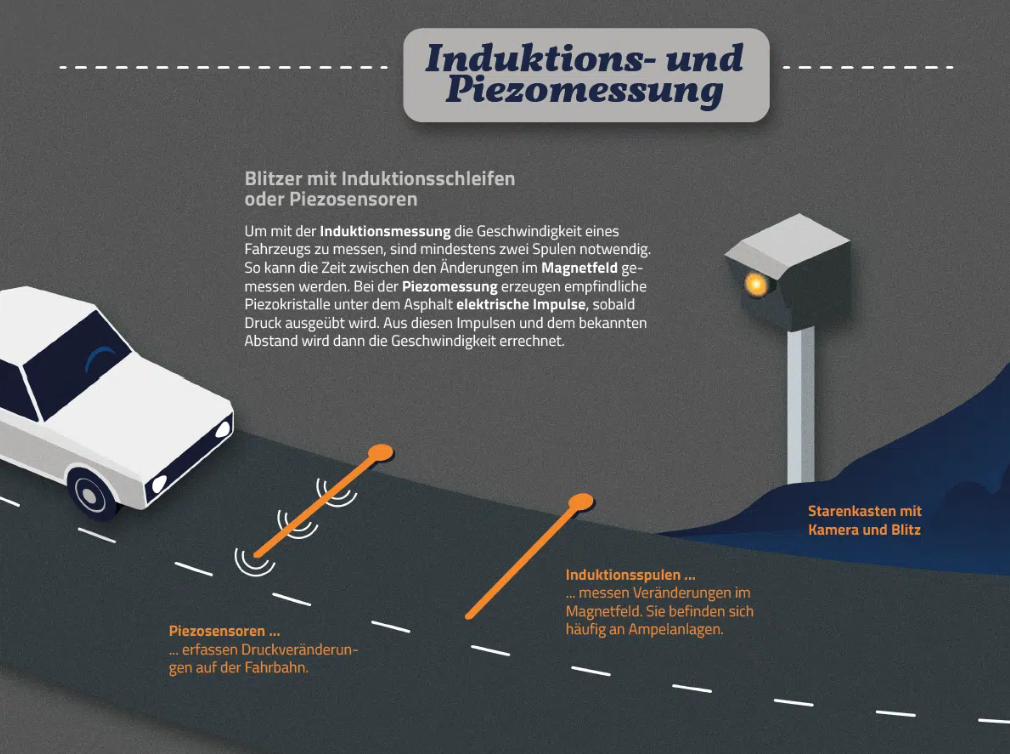
\includegraphics[width=0.85\linewidth]{Bilder/Blitzer_induktionsmessung.png}\\
\footnotesize Blitzer mit Induktionsschleifen
\end{minipage}%
\hfill
\begin{minipage}[t]{0.47\linewidth}
\centering
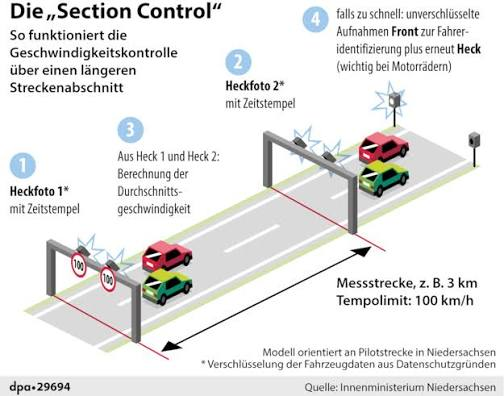
\includegraphics[width=0.85\linewidth]{Bilder/abschnittkontrolle.jpg}\\
\footnotesize Abschnittskontrolle
\end{minipage}
\end{center}

% Lehrperson: Hier innehalten und die Klasse überlegen lassen, bevor die
% Theoriebox unten die Auflösung liefert. Leitfragen: Was genau misst
% jedes der beiden Geräte? Über welche Distanz? Was könnte ein Vorteil der
% Abschnittskontrolle gegenüber dem Blitzer sein?

Was, glaubt ihr, misst jedes der beiden Geräte genau, und über welche
Distanz? Und was könnte ein Vorteil der Abschnittskontrolle gegenüber
einem einzelnen Blitzer sein? Haltet eure Vermutung kurz in Stichworten
fest.
\Antwortraum{1}
\end{beispielbox}

\needspace{45\baselineskip}
\begin{questions}
\begin{taskbox}[Übung: Blitzer oder Abschnittskontrolle im Diagramm]
\question[10] Ein Auto durchfährt eine Autobahnbaustelle (Tempolimit
$\SI{80}{\kilo\meter\per\hour}$). Am Anfang und am Ende der Baustelle
steht je eine Kamera einer Abschnittskontrolle; irgendwo dazwischen steht
zusätzlich ein einzelner Blitzer. Das folgende $s$-$t$-Diagramm zeigt die
Fahrt durch die gesamte Baustelle.

\begin{center}
\begin{tikzpicture}[scale=0.85]
  \draw[gray!20] (0,0) grid[xstep=1,ystep=1] (6,8.5);
  \draw[->] (-0.3,0) -- (6.7,0) node[right] {\scriptsize $t$ in min};
  \draw[->] (0,-0.3) -- (0,9.3) node[above] {\scriptsize $s$ in km};
  \foreach \x/\lbl in {2/10,2.6/13,6/30} \draw (\x,0.08) -- (\x,-0.08) node[below] {\scriptsize \lbl};
  \foreach \y/\lbl in {3/12,4.25/17,8.5/34} \draw (0.08,\y) -- (-0.08,\y) node[left] {\scriptsize \lbl};
  \draw[thick,titleblue] (0,0) -- (2,3) -- (2.6,4.25) -- (6,8.5);
  \filldraw[black] (0,0) circle (1.8pt);
  \filldraw[black] (2,3) circle (1.8pt);
  \filldraw[black] (2.6,4.25) circle (1.8pt);
  \filldraw[black] (6,8.5) circle (1.8pt);
\end{tikzpicture}
\end{center}

\begin{parts}
  \part[3] Bestimme die Geschwindigkeit des Autos in jedem der drei
  Fahrtabschnitte in $\si{\kilo\meter\per\hour}$.
  \Antwortraum{3}
  \begin{solution}
  Abschnitt 1 ($t=0$ bis $\SI{10}{\minute}$):
  \[
    v_1 = \frac{\SI{12}{\kilo\meter}}{\SI{10}{\minute}} = \frac{\SI{12}{\kilo\meter}}{\frac{10}{60}\,\si{\hour}} = \SI{72}{\kilo\meter\per\hour}.
  \]
  Abschnitt 2 ($t=\SI{10}{\minute}$ bis $\SI{13}{\minute}$):
  \[
    v_2 = \frac{\SI{17}{\kilo\meter}-\SI{12}{\kilo\meter}}{\SI{13}{\minute}-\SI{10}{\minute}} = \frac{\SI{5}{\kilo\meter}}{\frac{3}{60}\,\si{\hour}} = \SI{100}{\kilo\meter\per\hour}.
  \]
  Abschnitt 3 ($t=\SI{13}{\minute}$ bis $\SI{30}{\minute}$):
  \[
    v_3 = \frac{\SI{34}{\kilo\meter}-\SI{17}{\kilo\meter}}{\SI{30}{\minute}-\SI{13}{\minute}} = \frac{\SI{17}{\kilo\meter}}{\frac{17}{60}\,\si{\hour}} = \SI{60}{\kilo\meter\per\hour}.
  \]
  \end{solution}

  \part[2] In welchem Abschnitt (falls überhaupt) wird das Auto vom
  Blitzer geblitzt? Begründe.
  \Antwortraum{2}
  \begin{solution}
  In Abschnitt 2: $v_2=\SI{100}{\kilo\meter\per\hour} >
  \SI{80}{\kilo\meter\per\hour}$ (Tempolimit). In den Abschnitten 1 und 3
  liegt die Geschwindigkeit unter dem Limit, dort löst ein Blitzer nicht
  aus.
  \end{solution}

  \part[3] Stellt die Abschnittskontrolle für die gesamte dargestellte
  Fahrt (Start bis Ende der Baustelle) eine Busse aus? Begründe mit einer
  Rechnung.
  \Antwortraum{3}
  \begin{solution}
  Gesamtstrecke $\Delta s=\SI{34}{\kilo\meter}$, Gesamtzeit
  $\Delta t=\SI{30}{\minute}=\SI{0.5}{\hour}$.
  \[
    \bar v = \frac{\Delta s}{\Delta t} = \frac{\SI{34}{\kilo\meter}}{\SI{0.5}{\hour}} = \SI{68}{\kilo\meter\per\hour}.
  \]
  Da $\SI{68}{\kilo\meter\per\hour} < \SI{80}{\kilo\meter\per\hour}$,
  stellt die Abschnittskontrolle \textbf{\emph{keine}} Busse aus.
  \end{solution}

  \part[2] Wie ist es möglich, dass das Auto in Abschnitt 2 geblitzt
  wird, die Abschnittskontrolle für die gesamte Fahrt aber keine Busse
  ausstellt?
  \Antwortraum{2}
  \begin{solution}
  Der Blitzer misst punktuell genau in Abschnitt 2, wo das Tempolimit
  tatsächlich kurzzeitig überschritten wird. Die Abschnittskontrolle
  mittelt dagegen über die ganze, viel längere Fahrt: Da das Auto in den
  beiden anderen Abschnitten deutlich langsamer als das Limit fährt,
  gleicht das die kurze Überschreitung in der Durchschnittsgeschwindigkeit
  über die gesamte Strecke wieder aus.
  \end{solution}
\end{parts}
\end{taskbox}
\end{questions}

% --- Marathon-Beispiel: gleiche Durchschnittsgeschwindigkeit, ganz
% unterschiedlicher Momentangeschwindigkeits-Verlauf.
\begin{beispielbox}[Beispiel: Drei Läuferinnen und Läufer am Zürich Marathon]
Sofia, Elias und Noa laufen gemeinsam den Zürich Marathon (Streckenlänge
gerundet $\SI{42}{\kilo\meter}$).

\begin{center}
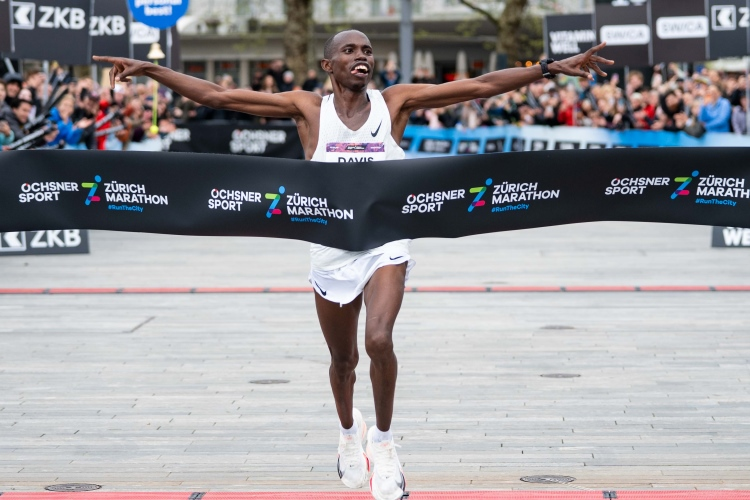
\includegraphics[width=0.55\linewidth]{Bilder/zurich_marathon.jpg}\\
\footnotesize Zürich Marathon
\end{center}

\begin{itemize}[leftmargin=1.2cm,itemsep=0.4em]
  \item \textbf{Sofia} läuft das ganze Rennen durch, in einem sehr
  gleichmässigen Tempo.
  \item \textbf{Elias} legt bei einem Verpflegungsposten eine kurze Pause
  ein, um zu trinken und zu essen. Danach läuft er bewusst schneller, um
  den Rückstand aufzuholen, und erreicht schliesslich zur exakt
  gleichen Zeit wie Sofia die Ziellinie, direkt neben ihr.
  \item \textbf{Noa} muss unterwegs dringend auf die Toilette und legt
  dafür ebenfalls einen Stopp ein. Anders als Elias schafft sie es aber
  nicht mehr, den entstandenen Rückstand aufzuholen: Als Sofia und Elias
  ins Ziel laufen, ist Noa noch ein Stück von der Ziellinie entfernt.
\end{itemize}
\end{beispielbox}

\needspace{50\baselineskip}
\begin{questions}
\begin{taskbox}[Übung: Alle drei im gleichen $s$-$t$-Diagramm]
\question[12] Betrachte den Zeitraum vom Start ($t=\SI{0}{\minute}$,
$s=\SI{0}{\kilo\meter}$) bis zu dem Moment, in dem Sofia die Ziellinie
erreicht. Für jede Person sind unten die einzelnen Abschnitte ihrer
Bewegung (Dauer und Geschwindigkeit) gegeben.

\begin{center}
\begin{tabular}{@{}llcc@{}}
\toprule
\textbf{Person} & \textbf{Abschnitt} & \textbf{Dauer} & \textbf{Geschwindigkeit}\\
\midrule
Sofia & gesamtes Rennen & $\SI{210}{\minute}$ & $\SI{12}{\kilo\meter\per\hour}$\\
\midrule
Elias & 1: bis Verpflegungsposten & $\SI{105}{\minute}$ & $\SI{12}{\kilo\meter\per\hour}$\\
 & 2: Pause & $\SI{15}{\minute}$ & $\SI{0}{\kilo\meter\per\hour}$\\
 & 3: Aufholen & $\SI{90}{\minute}$ & $\SI{14}{\kilo\meter\per\hour}$\\
\midrule
Noa & 1: bis WC-Stopp & $\SI{75}{\minute}$ & $\SI{12}{\kilo\meter\per\hour}$\\
 & 2: WC-Stopp & $\SI{15}{\minute}$ & $\SI{0}{\kilo\meter\per\hour}$\\
 & 3: nach dem Stopp & $\SI{120}{\minute}$ & $\SI{12}{\kilo\meter\per\hour}$\\
\bottomrule
\end{tabular}
\end{center}

\begin{parts}
  \part[6] Berechne für jeden Abschnitt jeder Person die zurückgelegte
  Strecke $\Delta s = v\cdot\Delta t$ und damit, bei welcher Position $s$
  jeder Abschnitt endet.
  \Antwortraum{6}
  \begin{solution}
  \textbf{Sofia:} $\Delta s = \SI{12}{\kilo\meter\per\hour}\cdot\SI{3.5}{\hour} = \SI{42}{\kilo\meter}$ (Ende bei $t=\SI{210}{\minute}$, $s=\SI{42}{\kilo\meter}$).

  \textbf{Elias:} Abschnitt 1: $\Delta s = \SI{12}{\kilo\meter\per\hour}\cdot\SI{1.75}{\hour} = \SI{21}{\kilo\meter}$ (bei $t=\SI{105}{\minute}$: $s=\SI{21}{\kilo\meter}$).
  Abschnitt 2: $\Delta s = \SI{0}{\kilo\meter}$ (bei $t=\SI{120}{\minute}$: $s=\SI{21}{\kilo\meter}$).
  Abschnitt 3: $\Delta s = \SI{14}{\kilo\meter\per\hour}\cdot\SI{1.5}{\hour} = \SI{21}{\kilo\meter}$ (bei $t=\SI{210}{\minute}$: $s=\SI{42}{\kilo\meter}$).

  \textbf{Noa:} Abschnitt 1: $\Delta s = \SI{12}{\kilo\meter\per\hour}\cdot\SI{1.25}{\hour} = \SI{15}{\kilo\meter}$ (bei $t=\SI{75}{\minute}$: $s=\SI{15}{\kilo\meter}$).
  Abschnitt 2: $\Delta s = \SI{0}{\kilo\meter}$ (bei $t=\SI{90}{\minute}$: $s=\SI{15}{\kilo\meter}$).
  Abschnitt 3: $\Delta s = \SI{12}{\kilo\meter\per\hour}\cdot\SI{2}{\hour} = \SI{24}{\kilo\meter}$ (bei $t=\SI{210}{\minute}$: $s=\SI{39}{\kilo\meter}$).
  \end{solution}

  \part[6] Zeichne für alle drei Personen das vollständige (stückweise
  lineare) $s$-$t$-Diagramm in das folgende \textbf{gemeinsame}
  Koordinatensystem ein. Beschrifte jede Linie.

  \begin{center}
  \begin{tikzpicture}[scale=0.8]
    \draw[gray!25] (0,0) grid[xstep=1,ystep=1] (14,14);
    \draw[->] (-0.3,0) -- (14.7,0) node[right] {\scriptsize $t$ in min};
    \draw[->] (0,-0.3) -- (0,14.7) node[above] {\scriptsize $s$ in km};
    \foreach \x/\lbl in {1/15,2/30,3/45,4/60,5/75,6/90,7/105,8/120,9/135,10/150,11/165,12/180,13/195,14/210} \draw (\x,0.06) -- (\x,-0.06) node[below] {\scriptsize \lbl};
    \foreach \y/\lbl in {1/3,2/6,3/9,4/12,5/15,6/18,7/21,8/24,9/27,10/30,11/33,12/36,13/39,14/42} \draw (0.06,\y) -- (-0.06,\y) node[left] {\scriptsize \lbl};
  \end{tikzpicture}
  \end{center}

  \begin{solution}
  \begin{center}
  \begin{tikzpicture}[scale=0.8]
    \draw[gray!25] (0,0) grid[xstep=1,ystep=1] (14,14);
    \draw[->] (-0.3,0) -- (14.7,0) node[right] {\scriptsize $t$ in min};
    \draw[->] (0,-0.3) -- (0,14.7) node[above] {\scriptsize $s$ in km};
    \foreach \x/\lbl in {1/15,2/30,3/45,4/60,5/75,6/90,7/105,8/120,9/135,10/150,11/165,12/180,13/195,14/210} \draw (\x,0.06) -- (\x,-0.06) node[below] {\scriptsize \lbl};
    \foreach \y/\lbl in {1/3,2/6,3/9,4/12,5/15,6/18,7/21,8/24,9/27,10/30,11/33,12/36,13/39,14/42} \draw (0.06,\y) -- (-0.06,\y) node[left] {\scriptsize \lbl};
    \draw[thick,titleblue] (0,0) -- (14,14);
    \draw[thick,accentorange] (0,0) -- (7,7) -- (8,7) -- (14,14);
    \draw[thick,accentpurple] (0,0) -- (5,5) -- (6,5) -- (14,13);
    \filldraw[black] (14,14) circle (2pt) node[above left,xshift=-1mm] {\scriptsize Sofia/Elias: Ziel};
    \filldraw[black] (14,13) circle (2pt) node[below left,yshift=-1mm] {\scriptsize Noa};
  \end{tikzpicture}\\
  \footnotesize \textcolor{titleblue}{Sofia} (gleichmässig), \textcolor{accentorange}{Elias} (Pause bei $t=\SI{105}{\minute}$, holt danach steiler auf und trifft Sofia genau im Ziel wieder), \textcolor{accentpurple}{Noa} (Pause bei $t=\SI{75}{\minute}$, läuft danach parallel zu Sofia weiter und bleibt deshalb dauerhaft zurück).
  \end{center}
  \end{solution}
\end{parts}
\end{taskbox}
\end{questions}

\needspace{40\baselineskip}
\begin{questions}
\begin{taskbox}[Übung: Momentan- vs. Durchschnittsgeschwindigkeit beim Marathon]
\question[6] Vergleiche für jede Person die Momentangeschwindigkeit
$v(t)$ während des Rennens mit ihrer Durchschnittsgeschwindigkeit $\bar
v$ über das ganze Rennen, und beziehe dich dabei auf das Diagramm, das
ihr oben gezeichnet habt.

\begin{parts}
  \part[2] Wie verhält sich Sofias Momentangeschwindigkeit im Vergleich
  zu ihrer Durchschnittsgeschwindigkeit?
  \Antwortraum{2}
  \begin{solution}
  Da Sofia sehr gleichmässig läuft, ist ihre Momentangeschwindigkeit zu
  fast jedem Zeitpunkt ungefähr gleich gross wie ihre
  Durchschnittsgeschwindigkeit über das ganze Rennen: $v(t)\approx\bar
  v_{\text{Sofia}}$.
  \end{solution}

  \part[2] Wie verhält sich Elias' Momentangeschwindigkeit in den
  einzelnen Abschnitten im Vergleich zu seiner Durchschnittsgeschwindigkeit
  über das ganze Rennen, und wie ist es möglich, dass seine Linie im
  Diagramm oben trotzdem am selben Punkt endet wie Sofias?
  \Antwortraum{2}
  \begin{solution}
  In Abschnitt 1 entspricht Elias' Momentangeschwindigkeit
  ($\SI{12}{\kilo\meter\per\hour}$) etwa seiner späteren
  Durchschnittsgeschwindigkeit. In Abschnitt 2 (Pause) ist sie $v(t)=0$,
  deutlich darunter -- die Linie verläuft dort waagrecht. In Abschnitt 3
  ist sie mit $\SI{14}{\kilo\meter\per\hour}$ grösser als sein
  Durchschnitt, die Linie ist dort steiler als in Abschnitt 1 und auch
  steiler als Sofias durchgehende Linie. Genau dieser steilere Abschnitt
  gleicht die während der Pause verlorene Zeit wieder aus, sodass Elias
  trotz des ganz anderen Bewegungsverlaufs am Ende exakt im selben Punkt
  wie Sofia ankommt.
  \end{solution}

  \part[2] Wie verhält sich Noas Bewegung nach dem WC-Stopp im Vergleich
  zu Elias' Aufholphase, und weshalb bleibt sie deshalb dauerhaft hinter
  Sofia und Elias zurück?
  \Antwortraum{2}
  \begin{solution}
  Nach dem WC-Stopp läuft Noa in Abschnitt 3 wieder mit derselben
  Geschwindigkeit wie vorher ($\SI{12}{\kilo\meter\per\hour}$), anders
  als Elias läuft sie danach nicht schneller. Ihre Linie verläuft ab dort
  deshalb \emph{parallel} zu Sofias Linie, mit demselben Abstand wie beim
  Ende des WC-Stopps: Der während der Pause entstandene Rückstand wird
  nie mehr aufgeholt. Deshalb bleibt Noas Linie im Diagramm oben
  durchgehend unterhalb der anderen beiden und endet bei
  $t=\SI{210}{\minute}$ noch vor der Ziellinie.
  \end{solution}
\end{parts}
\end{taskbox}
\end{questions}

\end{document}
